\section{Digital Image Fundamentals}

영상처리는 Image acquisition - Image enhancement(e.g., 이미지의 명도, 대비를 조정) - Image restoration(e.g., 이미지의 품질을 개선) - Morphological processing(e.g., 컴퓨터가 인식하기 좋은 형태로 이미지 가공) - segmentation - object recognition - representation 스테이지를 거친다.

\subsection{Image Formation in the Eye}

이미지는 특정한 시각에 특정한 방향을 봤을 때 나타나는 시각적 자극을 단편적으로 표현한 것. 즉, 실세계에 있는 물체를 재현해 사람으로 하여금 같은 물체로 인식하도록 자극을 주는 것이다. 사람 눈이 정확하지 않기 때문에 경계선이 밝아보이는 Mach-band effect, simultaneous contrast 등 착시와 왜곡이 발생.

이미지는 2차원 상의 한 점을 받는 함수, $f(x, y)$로 표현할 수 있다. 래스터 이미지는 모든 $(x, y)$에 대한 $f$ 값을 알면 된다는 발상. 모든 픽셀의 intensity를 저장해두는 것이 래스터. reproduce하기 쉽고 전역적으로 변경하기 쉽다. 하지만, 파일 크기가 커지고 확대하면 픽셀이 보이는 문제가 있다. 반면 벡터는 지정해둔 점을 잇는 방식.

\subsection{Lights}

전자기파의 성질은 반사. 물체를 본다는 것은 광원으로부터 나온 전자기파가 물체에 부딪혀 반사된 것을 눈의 신경을 거쳐 뇌에 전달되는 것. 물체는 빛의 일부를 흡수해서 열로 전이하고, 일부는 반사/분산시킨다.

\subsection{Image Acquisition}

빛을 전기 신호로 변환하는 센서가 있음.

\bitmz
  \itm Single Element Sensing: 하나의 센서가 움직이며 회전하는 필름을 스캔하는 방식. 센서 이동 속도를 조절하면 해상도를 조절할 수 있다. 천천히 움직일수록 해상도가 높아진다. 하지만 느리다.
  \itm Sensor Strip Sensing: 센서를 일렬로 붙여놓은 스트립을 움직이며 스캔하는 방식. 스트립을 처음 만들 때 붙인 센서 수에 따라 해상도가 결정된다. 복사기 스캐너, CT가 예시.
  \itm 2D Image Array Sensing: 센서를 2차원 배열로 이어붙인 형태. 스냅샷을 얻을 수 있다는 특징이 있음. 대량 생산되고 있기 때문에 단일 센서보다 저렴해졌다. 한번 센서 배열을 만들면 해상도를 높일 수 없다는 단점이 있음.
\eitmz

이미지를 디지털로 처리하려면 연속적인 빛을 이산적으로 취해야 한다. 그 과정은 아래와 같다.

\benum
  \itm 광원으로부터 $I$ 방향으로 물체에 빛이 들어온다.
  \itm 반사율 $r$에 따라 $d$ 방향으로 빛이 반사된다.
  \itm 반사된 빛이 렌즈를 거쳐 CCD(Charge coupled device)의 어떤 점 $(x, y)$에 도달한다.
\eenum

\bitmz
  \itm $f(x, y)$: 어떤 $(x, y)$ 좌표가 주어지면 그 위치의 밝기(intensity)를 반환한다.
  \itm $L_{min} \leq l \leq L_{max}$:  센서가 처리할 수 있는 최소/최대의 밝기가 한정되어 있다.
  \itm $[L_{min}, L_{max}]$ 범위. 일반적으로 $[0, L - 1]$ 범위를 갖는다. 0부터 시작했기 때문에 최대는 $L$이 아니라 $L - 1$이 된다. (e.g., [0, 255])
\eitmz

\subsection{Sampling and Quantization (Digitalization)}

샘플링(Sampling): 컴퓨터가 실세계의 빛을 모두 저장해 처리할 수 없으므로, 연속적으로 변화하는 실세계의 데이터에서 일부를 취하는 것. 무조건 많이 하는 것이 좋다. 이미지의 모든 $f(x, y)$를 저장할 수 없으니 몇 개의 점에 대한 $f$ 값을 선택해 저장하는 것: $f(x, y) \Rightarrow f(x_i, y_j)$.

양자화(Quantization): 컴퓨터가 데이터를 이산적으로 취급하므로, 연속적인 실수 값을 정수 값으로 변환해 이산적인 값을 얻는 것. 이렇게 얻은 밝기 값의 범위를 $[0, L - 1]$라고 하면, 2진수로 저장하므로 $L = 2^k$. $M \times N$ 크기 디지털 이미지를 저장하기 위한 비트의 개수 $b = M \times N \times k$. 양자화로 인해 saturation 문제가 발생. 가령 255보다 밝은 부분을 표현하려면 어쩔 수 없이 255로 저장해야 한다.

\begin{figure}[h]
  \centering
  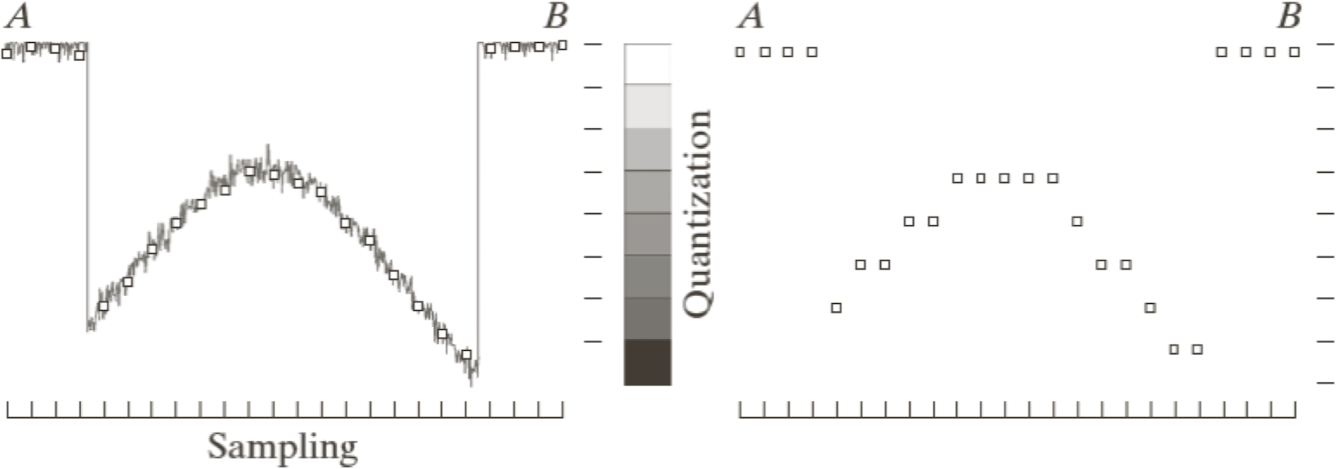
\includegraphics[width=\columnwidth]{sampling-and-quantization.png}
\end{figure}

샘플링은 x축에 대한 적용이고, 양자화는 y축에 대한 적용이라고 생각하면 된다.

\subsection{Image Interpolation}

알고 있는 데이터를 이용해 모르는 값을 추정하는 것. 예를 들어 2x2 이미지를 8x8로 확대한다면 아는 픽셀 값을 이용해 모르는 픽셀 값을 채워야 한다.

\bitmz
  \itm Nearest neighbor interpolation: $v(x, y) = f(round(x), round(y))$. 특정 픽셀에서 가장 가까운 픽셀의 값을 사용. 계산이 빠르지만 개체의 경계가 망가지고 해상도가 낮아지는 문제.
  \itm Bilinear interpolation: $v(x, y) = ax + by + cxy + d$. 인접한 4개 픽셀과 거리를 바탕으로 값을 결정.
  \itm Bicubic interpolation: $v(x, y) = \sum_{i=0}^3 \sum_{j=0}^3 a_{ij} x^i y^j$. 주변 16개 픽셀과 거리에 따른 가중치를 바탕으로 값을 결정. 보다 정교하게 보간할 수 있음.
\eitmz

\subsection{Relationship between Pixels}

어떤 픽셀 $(x, y)$가 주어졌을 때 주변 픽셀의 정의.

\bitmz
  \itm 4 neighbors ($N_4(p)$): 상하좌우 4개 픽셀.
  \itm 4 diagonal neighbors ($N_D(p)$): 대각선에 있는 4개 픽셀.
  \itm 8 neighbors ($N_8(p)$): 둘러싼 8개 픽셀.
\eitmz

주변 픽셀 중에서도 같은 속성을 가진 것을 adjacency라고 한다. adjacency끼리 연결하면 path가 만들어짐. 두 픽셀이 connected되어 있다는 것은 두 픽셀 사이에 path가 존재한다는 것. connected 픽셀들의 서브셋을 region이라고 한다.

Boundary: 경계선. 특정 픽셀의 바로 옆에 다른 region이 나온다면 그 픽셀이 boundary라고 할 수 있다. boundary 픽셀을 포함해서 region으로 취급한다면 inner border, 그렇지 않다면 outer border.

Distance Measure: 거리를 metric하게 구한다는 것은: (1) 거리가 양수 ($D(p, q) \geq 0$). 이때 p와 q가 같다면 $D(p, q) = 0$, (2) p에서 q까지의 거리가 q에서 p까지의 거리와 같음 ($D(p, q) = D(q, p)$), (3) p에서 z까지의 거리가 p에서 q를 거친 z까지의 거리보다 짧거나 같음 ($D(p, z) \leq D(p, q) + D(q, z)$). 아래와 같은 metrics가 있음.

\bitmz
  \itm Euclidean: $D_e(p, q) = \sqrt{(x - s)^2 + (y - t)^2}$
  \itm Manhattan: $D_4(p, q) = |x - s| + |y - s|$
  \itm Chessboard: $D_8(p, q) = \max(|x - s|, |y - t|)$
\eitmz

\subsection{Mathematical Tools}

$f(x, y)$ 이미지를 $g(x, y)$ 이미지로 변환한다. 이때 $H$는 영상처리 함수.
$$
H[f(x, y)] = g(x, y)
$$
Linear Operation: $f_i(x, y)$ 이미지의 모든 픽셀에 $a_i$를 곱한 값에 $f_j(x, y)$ 이미지의 모든 픽셀에 $a_j$를 곱한 값을 더한다. $H$ 연산을 한 번만 해도 된다는 점에 의의가 있음.
$$
\begin{aligned}
  H[a_i f_i(x, y) &+ a_j f_j(x, y)] \\
  &= a_i H[f_i(x, y)] + a_j H[f_j(x, y)] \\
  &= a_i g_i(x, y) + a_j g_j(x, y)
\end{aligned}
$$
몇몇 arithmtic operation이 있음.

\bitmz
  \itm Addition: $s(x, y) = f(x, y) + g(x, y)$.
  \itm Subtraction: $s(x, y) = f(x, y) - g(x, y)$. $[0, L - 1] - [0, L - 1]$ 연산을 하면 $[-L - 1, 0]$이 될 수 있기 때문에 주의해야.
  \itm Multiplication: $s(x, y) = f(x, y) \times g(x, y)$.
  \itm Division: $s(x, y) = f(x, y) \div g(x, y)$. 밝기가 일정한 이미지가 얻어짐.
\eitmz

logical operation도 가능하다.

\section{Intensity Transformations and Spatial Filtering}

기본적인 intensity transform은 $g(x, y) = T[f(x, y)]$. 딱 한 점만 가져오는 게 아니라 주변 점을 같이 확인한다.

\bitmz
  \itm Averaging neighbor pixels: $g(x, y) = T[f(x, y)]$.
  \itm 4 neighbor: $g(x, y) = {1 \over 5} (f(x, y) + f(x + 1, y) + f(x - 1, y) + f(x, y + 1) + f(x, y - 1))$.
  \itm 8 neighbor: ${1 \over 9} \sum_{i=-1}^1 \sum_{j=-1}^1 f(x + i, y + j)$.
\eitmz

$g(x, y)$ 픽셀을 계산하기 위해 $f(x, y)$에 3x3 윈도우를 적용한다.

\subsection{Intensity Transformation Functions}

가장 작은 neighborhood 크기는 1x1. $s = T(r)$, Gray-level function 또는 Mapping function이라고 한다. 다양한 변환 함수가 있다.

\bitmz
  \itm Negatives: $s = L - 1 - r$. 어두운 이미지의 역상(negative)를 계산해 밝게 만든다.
  \itm Log transform: $s = c\log(1 + r)$. $1 + r$에 $\log$를 취하면 어두운 부분은 밝아지고, 밝은 부분은 크게 변하지 않는다. $c$를 파라미터로 강도를 조절할 수 있다.
  \itm Power-Law(Gamma) transform: $s = cr^\gamma$. $\gamma < 1$일 때는 어두운 부분이 밝아지고, $\gamma > 1$일 때는 어두운 부분이 완전히 어둡게 되고 밝은 부분은 밝기에 따른 차이가 분명해진다. 모니터는 실제 에너지 값을 반영하지 않게 때문에 이미지를 보면 조금 어둡게 느껴진다. 그래서 보통 모니터에 $1 \over 2.2$ 정도의 감마를 적용해둔다. \begin{figure}[h] \centering 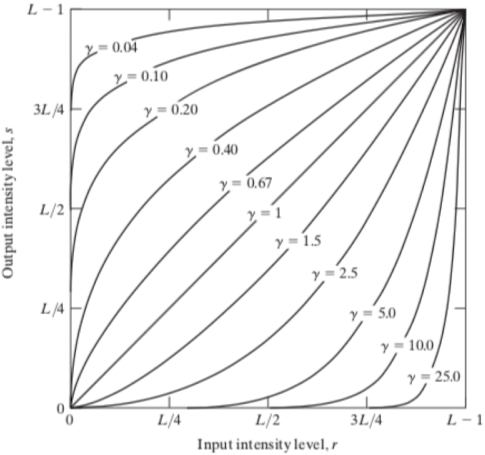
\includegraphics[width=7cm]{gamma-transform.png} \end{figure}
    \itm Piecewise-Linear transform: $s = ar + b$. a는 기울기(gain). a가 크면(기울기가 가파르면) contrast가 잘 보인다. b는 밝기(bias). b가 커지면서 s가 r보다 커지면 이미지가 밝아진다. 즉, contrast와 brightness가 항상 함께 조정된다. 특정 구간의 밝기만 조정하는 것은 intensity slicing.
\eitmz

\subsection{Histogram Processing}

히스토그램 분포가 고루 퍼져있어야 이미지가 잘 보인다고 간주할 수 있다. 따라서 histogram equalization을 한다. (사람이 보기에 항상 좋아지지는 않음. 그래도 밝은 이미지든, 어두운 이미지든 주변 밝기에 상관없이 일정한 값이 나오게 할 수 있다. 이렇게 해두면 다른 처리를 하기 편하다.) 이때, $s = T(r)$이고, $T(r)$은 엄격히 단조증가하는 함수라고 가정한다.

히스토그램을 확률 분포 함수로 간주한다. $p_r(r) = {H(r) \over {\sum_j H(j)}}$, 즉, 특정 픽셀 r의 히스토그램을 전체 히스토그램의 합으로 나눈 것. 좋은 히스토그램은 $p_s(s) = c$. 모든 픽셀이 동일한 상수. 이때 누적분포함수 $\text{cdf}_s(s) = {s \over L - 1}$.

이미지 전체에 histogram equalization을 하지 않고 일부분만 하는 것을 local(adaptive) histogram equlization(AHE)라고 한다. 이때 경계선이 어색하지 않도록 윈도우를 겹쳐서 쓴다.

\subsection{Spatial Filtering fundamentals}

spatial filtering은 이미지보다 작은 윈도우를 정의해 한 픽셀씩 이동하면서 필터를 적용하는 방식. 이렇게 이미지의 첫 픽셀부터 마지막 픽셀까지 커널의 입력 픽셀을 모두 곱해 합한 것을 컨볼루션(convolution)이라고 한다.

특정 픽셀을 중심으로 한 neighborhood의 집합과 해당 집합에 어떤 operation을 적용할지 정의해야 한다. 이때 시그마 부분은 neighborhood, 중심을 기준으로 $-a \sim a$, $-b \sim b$ 영역을 얻는다. $w(s, t)$ 부분은 operation.
$$
g(x, y) = \sum_{a=-1}^a \sum_{b=-1}^b w(s, t) f(x + s, y + t)
$$
커널이 이미지의 코너에 있을 때는 커널의 영역 일부가 이미지 밖으로 나가는 문제. 이때 중심의 주변부를 임의로 채우기 위해 padding을 한다. 이미지를 복사해서 값을 채워넣지 않고도 할 수 있다. 다양한 방식의 padding이 있다.

\begin{figure}[h]
  \centering
  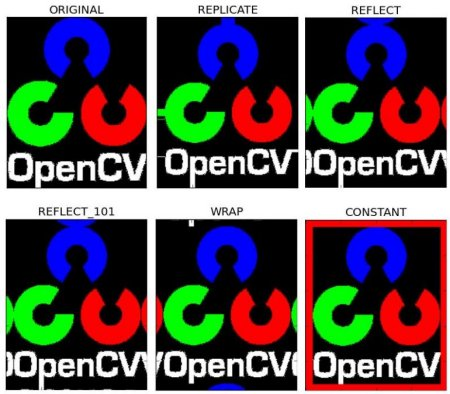
\includegraphics[width=\columnwidth]{padding.jpg}
\end{figure}

실제로 이미지를 키워서 임의의 픽셀을 채우는 방식이 아님. 커널의 영역이 유효하지 않은 위치를 참조하려 할 때, 패딩의 종류에 따른 값을 취하는 것일 뿐.

\subsection{Smoothing Spatial Filters}

노이즈를 제거하기 위한 필터.

\bitmz
  \itm Averaging filter: 윈도우 영역 내에 포함되는 픽셀들의 평균을 취하는 필터. 평균냄으로써 노이즈를 줄일 수 있다. 3x3 필터의 경우, $r(x, y) = {1 \over 9} \sum_{s=-1}^1 \sum_{t=-1}^1 f(x + s, y + t)$. 개체의 경계를 흐리게 만드는 단점이 있지만, 무의미한 디테일을 줄이는 데 사용할 수 있음. 윈도우 내 모든 픽셀의 가중치가 같은 경우 Box Filter라고 한다.
  \itm Weighted Averaging Filter: 중앙으로부터 거리가 멀수록 중요하지 않은 것으로 취급. 가우시안 커널을 사용한다: $w(s, t) = {1 \over 2\pi\sigma^2}e^{-{s^2 + t^2 \over \sigma^2}}$. 평균이 0이고, 표준편차가 1인 정규분포가 가우시안. $\sigma$가 커질수록 0에 가까워진다. 커널의 합이 1이 되도록(에너지를 보존하도록)하기 위해 임의의 값으로 나눠준다. 안 그러면 이미지가 전반적으로 밝아질 수 있음. $${1 \over 16} \times \begin{bmatrix} 1 & 2 & 1 \\ 2 & 4 & 2 \\ 1 & 2 & 1 \end{bmatrix}$$
  \itm Order-Statistic (Non-linear, Non-separable) Filter: 최대/최소/중앙값 필터. 가우시안으로는 노이즈가 없어지지 않고 형상이 뭉개지는 문제가 생길 수 있는데, 이때 사용한다. 중앙값 필터는 impulse (salt and pepper) noise를 없앨 수 있다. 후추(255)와 소금(0) 사이의 중앙값을 취함으로써 노이즈가 제거되는 것.
\eitmz

Separable Filter: 어떤 오퍼레이터는 separable하다. 각 필터를 따로 적용했을 때와 합쳐진 필터를 적용했을 때 결과가 같다. 가령 x방향으로 먼저 1D 필터링을 하고, y 방향으로 1D 필터링을 했을 때 2D 필터링과 같은 결과가 나온다. 거대한 커널에 operation을 하려면 $O(m \times n)$의 시간이 소요된다. 이때 separable filter를 사용하면 연산량을 줄여 $O(m + n)$으로 성능을 높일 수 있다. weighted averaging filter의 예시를 보면:
$$
{1 \over 4}
\begin{bmatrix}
  1 \\
  2 \\
  1
\end{bmatrix}
\ast {1 \over 4} [1 \; 2 \; 1] = {1 \over 16}
\begin{bmatrix}
  1 & 2 & 1 \\
  2 & 4 & 2 \\
  1 & 2 & 1
\end{bmatrix}
$$
예를 들어 DFT를 할 수 없는 상황에서 가우시안 필터링을 하는 경우, x축으로 1D 필터링을 한 다음 y축으로 1D 필터링을 하면 같은 결과를 얻으면서 더 나은 성능을 달성할 수 있다.

\subsection{Sharpening Spatial Filters}

smoothing 필터링과 반대로 이미지를 선명하게 만드는 필터. 기본 원리는 픽셀값이 변화하는 부분을 강조하는 것. 변화가 가장 큰 곳은 형상의 경계 부분이므로, 이미지를 미분해 경계를 알아내야 한다.

미분의 정의는 $\lim_{h \rightarrow 0} {f(x + h) - f(x) \over h}$. 하지만 픽셀 단위로 보면 값이 아무리 작아도 옆 픽셀이므로, 극한을 생략할 수 있다(finite difference). 따라서 이산적인 버전으로는 $f(x + 1) - f(x)$. 이때, 자신에게서 왼쪽 픽셀을 뺀 값($f(x) - f(x - 1)$)과 오른쪽 픽셀에서 자신을 뺀 값이 비슷하다.

\begin{figure}[h]
  \centering
  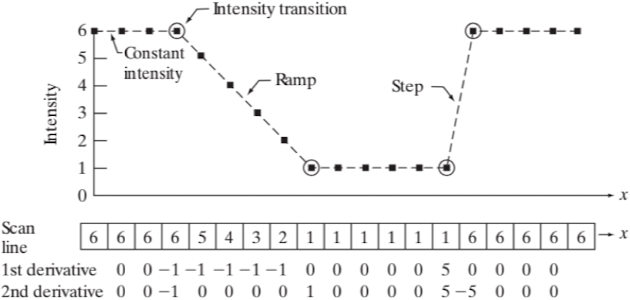
\includegraphics[width=\columnwidth]{derivatives-1.png}
\end{figure}

\begin{figure}[h]
  \centering
  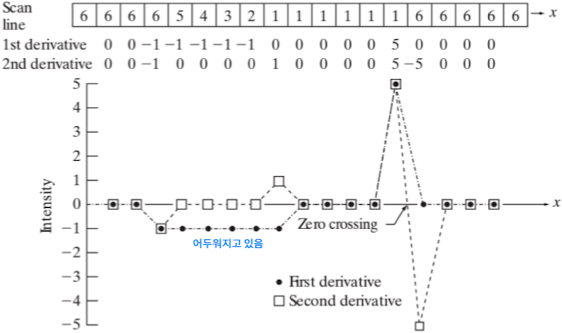
\includegraphics[width=\columnwidth]{derivatives-2.png}
\end{figure}

1차 미분(1st derivative)의 특성: (1) 픽셀값이 일정한 영역에서는 0, (2) 변화하고 있는 구간(step, ramp)에서는 non-zero, (3) ramp 구간에서는 non-zero.

2차 미분(2nd derivative)의 특성: (1) 픽셀값이 일정한 영역에서는 0, (2) 변화가 시작되는 지점에서는 non-zero, (3) 일정하게 변화하는 ramp 구간은 0. 갑자기 밝기가 급격하게 바뀌는 지점에서 0을 지나는 zero crossing이 발생한다.

이미지 전체에 2차 미분을 한 뒤 zero crossing이 일어나는 부분을 보면 경계를 찾을 수 있다.

\subsection{The Laplacian}

라플라시안 필터는 필터의 중심을 어떤 각도로 회전시켜도 동일한 필터가 유지되는 isotrophic 필터. x축으로 2차 미분, y축으로 2차 미분해서 더하면 된다. 2차원 이미지를 대상으로 2차 미분을 해야 하므로, 아래와 같이 정의할 수 있다. (보통 주변 4개의 픽셀을 본다.)
$$
\begin{aligned}
  \nabla^2 f &= {\partial^2 f \over \partial x^2} + {\partial^2 f \over \partial y^2} \\
  {\partial^2 f \over \partial x^2} &= f(x + 1, y) + f(x - 1, y) - 2f(x, y) \\
  {\partial^2 f \over \partial y^2} &= f(x, y + 1) + f(x, y - 1) - 2f(x, y) \\
  \therefore \nabla^2 f &= f(x + 1, y) + f(x - 1, y) \\
                        &+ f(x, y + 1) + f(x, y - 1) - 4(x, y)
\end{aligned}
$$
라플라시안의 특성: (1) intensity의 불연속적인 부분(경계선)을 강조, (2) intensity가 느리게 변화하는 영역의 강도 해제(deemphasizing).

라플라시안 커널은 다음과 같다. (각각 4-neighborhood, 8-neighborhood)
$$
\begin{bmatrix}
  0 & 1 & 0 \\
  1 & -4 & 1 \\
  0 & 1 & 0 \\
\end{bmatrix}
\;
\begin{bmatrix}
  1 & 1 & 1 \\
  1 & -8 & 1 \\
  1 & 1 & 1 \\
\end{bmatrix}
$$

샤프닝된 이미지를 $g(x, y)$라고 했을 때, 라플라시안 필터를 적용하는 것을 아래와 같이 표현할 수 있다.
$$g(x, y) = f(x, y) + c[\nabla^2 f(x, y)]$$
이렇게 라플라시안에 상수 $c$를 곱하고 원본 이미지를 더하면 경계 부분이 선명해진다.

\subsection{Unsharp Masking and Highboost Filtering}

이미지를 블러시켜 원본 이미지와 비교해 마스크를 얻는 방식. 블러는 빛이 변화하는 부분(경계선)을 부드럽게 만든다. 미분이 아니라 아래와 같은 방식으로 엣지를 찾는다.
\benum
  \itm 원본 이미지에 블러를 적용한다. (언샤프닝)
  \itm 블러링된 이미지와 원본 이미지 사이의 차이를 얻는다. (마스크)
  \itm 위에서 얻은 마스크를 원본 이미지에 더한다.
\eenum
원본 이미지가 $f(x, y)$, 블러된 이미지가 $\hat{f}(x, y)$라고 했을 때 이를 수식화하면,
$$
\begin{aligned}
  g_{mask}(x, y) &= f(x, y) - \hat{f}(x, y) \\
  g(x, y) &= f(x, y) + k \ast g_{mask}(x, y)
\end{aligned}
$$
$k$의 값에 따라 unsharp masking과 highboost filtering으로 나뉜다. $k = 1$인 경우 앞서 본 unsharp masking이고, $k > 1$인 경우 highboost filtering이다. highboost란 뭔가를 더 크게 강조한다는 것. $k$가 커질수록 경계선이 더욱 강조된다. $k < 1$인 경우 unsharp mask의 강조 효과가 약해지며, 음수가되면 그냥 블러와 비슷해진다.

\subsection{Gradient \& Sobel Operator}

isotrophic 필터인 라플라시안 필터가 2차 미분을 하는 것과 달리, anisotrophic filter는 1차 미분인 gradient를 사용한다.

Gradient: x축으로 미분한 것(자신의 오른쪽에서 자신을 뺀 것 or 자신에서 왼쪽을 뺀 것)과 y축으로 미분한 것을 묶어서 벡터로 표현한 것.
$$
\nabla f = grad(f) = \begin{bmatrix} g_x \\
g_y \end{bmatrix} = \begin{bmatrix} \partial f \over \partial x \\
\partial f \over \partial y \end{bmatrix}
$$
  gradient는 벡터이므로 방향과 크기를 갖는다. gradient의 방향은 이미지가 밝아지는 방향이고, 크기는 변화량이 얼마나 큰지(얼마나 빠르게 밝아지는지) 의미한다. 이때 벡터의 크기는 길이: $M(x, y) = mag(\nabla f) = \sqrt{g_x^2 + g_y^2}$. 이때 길이는 선형적이지 않다.

Sobel operator: gradient를 이용하는 필터. 기본적인 gradient는 $g_y = z_8 - z_5, g_x = z_6 - z_5$이지만, 이는 대칭적이지 않다. 대칭시키기 위해서는 양 옆을 서로 뺀 값을 쓴다. 그런데 한 픽셀끼리만 계산하면 변화가 급격해질 수 있으므로, 양 옆의 픽셀을 섞어서 노이즈의 영향을 줄인다. 이때 3x3 윈도우를 사용하면 아래와 같은 sobel operator가 된다.
$$
\begin{aligned}
  g_y &= {\partial f \over \partial y} = (z_7 + 2z_8 + z_9) - (z_1 + 2z_2 + z_3) \\
  g_x &= {\partial f \over \partial x} = (z_3 + 2z_6 + z_9) - (z_1 + 2z_4 + z_7)
\end{aligned}
$$
이때 커널의 총합은 0이 된다. 상대적인 값을 보려는 것이므로 $1 / 9$해줄 필요는 없다. sobel operator는 노이즈가 있는 영상에서 변화가 발생하는 경계 부분을 검출하는 데 특화되어 있다. 라플라시안이 날카롭게 경계를 검출한다면, sobel operator는 천천히 변화하는 영역에도 반응하기 때문에 비교적 부드럽게 경계가 추출된다.

여기까지 살펴본 여러 필터와 operation 중 하나만 사용하지 않고, 여러 레이어를 쌓아서 사용한다. 이렇게 하면 좋은 품질의 이미지를 만들 수 있다.

\section{Frequency Domain Processing}

모든 주기함수는 사인과 코사인의 합으로 표현할 수 있다. 주기함수는 $f(x) = f(x + c)$, 이때 모든 $x$에 대해 0이 아닌 상수 $c$가 존재하는 함수. 원본 주기함수의 주기보다 짧은 주기의 사인, 코사인 함수들을 섞어서 원본 함수를 만드는 것. 이때 어떤 주파수를 얼마나 적용할지 찾는 과정이 푸리에 변환.

\subsection{Fourier Series \& Transform}

복소수 $C$의 정의: $C = R + jI$. 이때 $R$, $I$는 실수, $j = \sqrt{-1}$. 복소수는 가로축이 실수부, 세로축이 허수부인 복소평면에 정의할 수 있음. 따라서 복소수 $R + jI$는 복소평면 상에서의 $(R, I)$와 같다.

\begin{figure}[h]
  \centering
  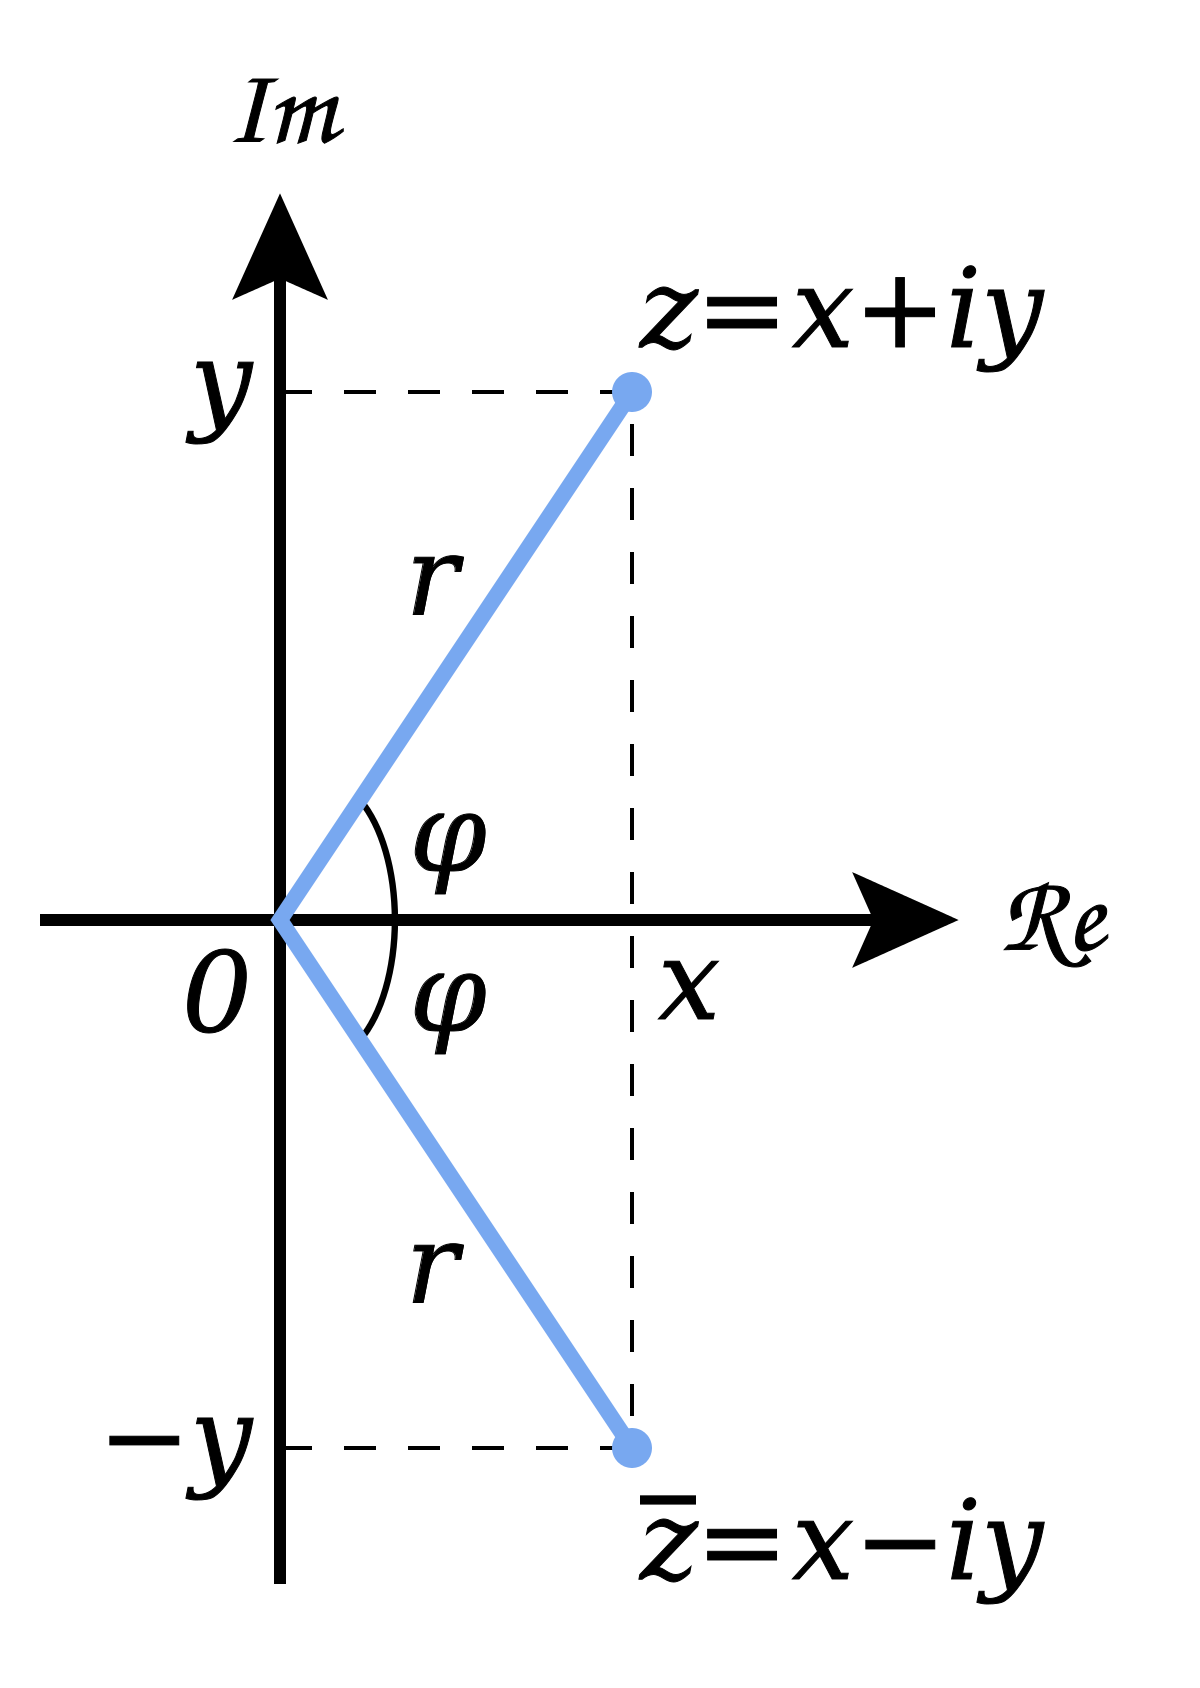
\includegraphics[width=4cm]{complex-plane.png}
\end{figure}

원점으로부터 복소수까지 직선을 그으면 길이와 각도가 생긴다. 즉, 극좌표계에서 표현할 수 있다.
$$C = |C|(\cos \theta + j \sin \theta)$$
이때 $\theta$는 가로축에서 직선까지의 각도, $|C|$는 원점으로부터 복소평면 상의 복소수까지의 거리. $|C| = \sqrt{R^2 + I^2}$. 여기에 오일러 공식 $e^{j \theta} = \cos \theta + j \sin \theta$를 적용하면 아래와 같이 간략히 쓸 수 있다.
$$C = |C|e^{j \theta}$$
복소평면에 표현할 수 있다는 것은 복소수를 함수로 표현할 수도 있다는 것.
$$
\begin{aligned}
  F(u) &= R(u) + jI(u) \\
  |F(u)| &= \sqrt{R(u)^2 + I(u)^2}
\end{aligned}
$$

\subsubsection{Implulse and their sifting property}

단위 임펄스는 아래와 같이 정의된다.
$$
\delta(t) =
\begin{cases}
  \infty & \text{if } t = 0 \\
  0 & \text{if } t \neq 0
\end{cases}
$$
컴퓨터는 이산적인 공간이므로, $\infty$가 아니라 1. 또한 $\sum_{x=-\infty}^{\infty} \delta(x) = 1$. $\Delta T$ 단위로 $n$만큼 평행이동 시킨 임펄스 함수들의 합은 impulse train을 형성한다: $s_{\Delta T}(t) = \sum_{n=-\infty}^\infty \delta(t - n\Delta T)$.

\begin{figure}[h]
  \centering
  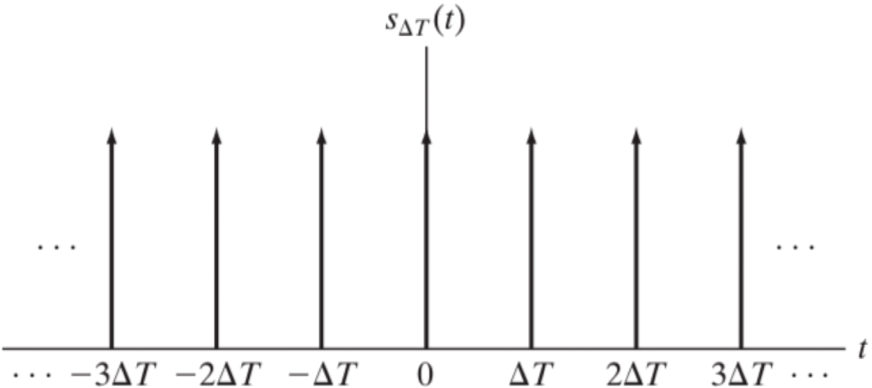
\includegraphics[width=\columnwidth]{impulse-train.png}
\end{figure}

\subsubsection{Image Transforms}

\begin{figure}[h]
  \centering
  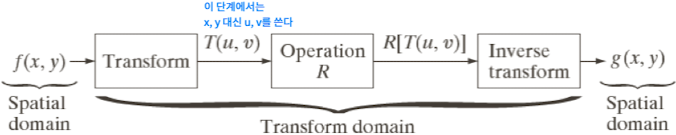
\includegraphics[width=\columnwidth]{image-transform-from-spatial-domain.png}
\end{figure}

spatial domain에서 다른 domain으로 이미지를 변환하여 operation을 수행한 뒤, 역변환하는 접근법. 이때 inverse transform은 아래와 같다.
$$f(t) = \int_{-\infty}^\infty F(\mu)e^{j2\pi \mu t}d\mu$$
$f(t)$는 다양한 주기함수를 모두 합쳐서 만들어진 코사인 함수. 여기서 $e^{j2\pi \mu t} = \cos 2\pi \mu t + j\sin 2\pi \mu t$. 따라서 $\mu$가 1일 때 $\theta$는 $2\pi t$, 2일 때는 $2\pi \times 2t$. 즉, $\mu$가 커질수록 한 사이클을 만들기 위한 거리가 줄어든다. $\mu$는 $t$가 0에서 1까지 갈 때 진동수(주기)를 의미.

주기는 $\mu$를 통해 알 수 있으므로 진폭만 알면 된다. $F$는 주기가 주어졌을 때 진폭을 반환하는 함수. inverse가 아니라 forward의 경우 $e$의 지수를 $-j2\pi \mu t$로 하면 된다.

\subsubsection{Convolution}

convolution의 정의는 아래와 같음. spatial filtering과 매우 유사하다.
$$f(t) \ast h(t) = \int_{-\infty}^\infty f(\tau)h(t - \tau)d\tau$$
convolution의 푸리에 변환은 아래와 같다.
$$
\begin{aligned}
  \Im\{f(t) \ast h(t)\} &= \\
  \int_{-\infty}^\infty &[\int_{-\infty}^\infty f(\tau)h(t - \tau)d\tau]e^{-j2\pi \mu t}d\tau \\
  H(\mu) &= \Im\{h(t - \tau)\} \Rightarrow H(\mu)e^{-j2\pi \mu t} \\
  H(\mu) \int_{-\infty}^\infty f(\tau)e^{-j2\pi \mu t}d\tau &= H(\mu) F(\mu)
\end{aligned}
$$
따라서 $f(t) \ast h(t) \Leftrightarrow H(\mu) F(\mu)$가 성립한다.

\subsection{Sampling \& Fourier Transform of Sampled Functions}

샘플링은 전체 이미지를 대표하는 몇 개 픽셀을 취하는 것. 수식으로는 아래와 같이 표현한다.
$$
\begin{aligned}
  \hat{f}(t) &= f(t)s_{\Delta T}(t) \\
  &= \sum f(t) \delta(t - n\Delta T) \\
  f_k &= f(k\Delta T)
\end{aligned}
$$
원본 신호에 impulse train을 곱하면 샘플링된다.

\begin{figure}[h]
  \centering
  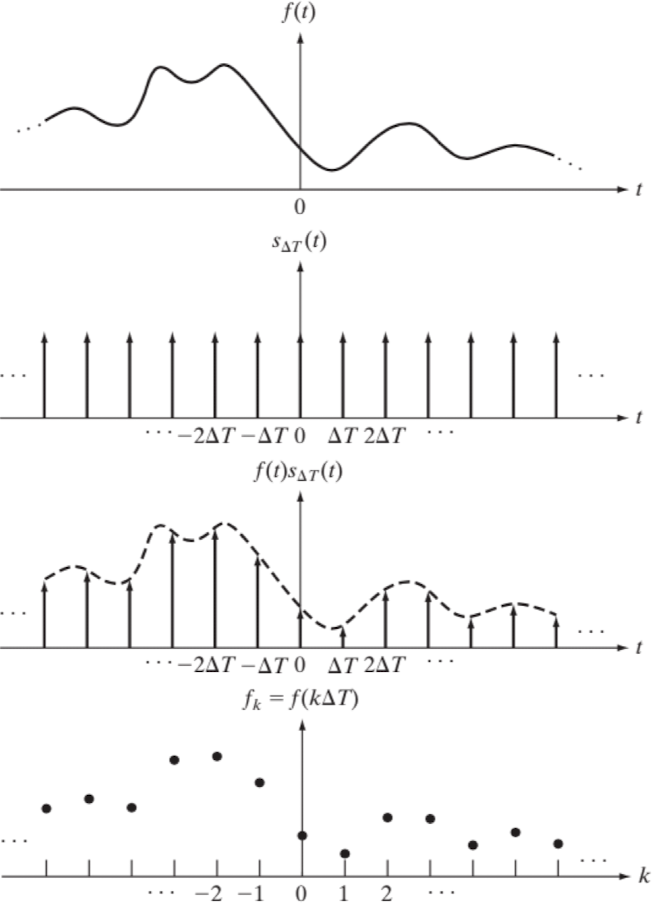
\includegraphics[width=6.4cm]{sampling.png}
\end{figure}

샘플링은 원본 신호에 따라 다르게 해야 한다. 이미지의 원본 형태를 유지하려면, 원본 신호가 가진 주파수의 최대값을 $\mu_{\text{max}}$라고 했을 때, 그 두 배를 샘플링해야 한다: ${1 \over \Delta T} > 2 \mu_{\text{max}}$. 샘플링을 그보다 적게하면 모아레 효과가 일어난다. 샘플링을 충분히 하지 않아서 원본 이미지에는 존재하지 않는 줄무늬 패턴이 보이는 것. 신호의 관점에서는 앨리어싱 문제임.

\subsection{Discrete Fourier Transform(DFT)}

이산함수에 대한 푸리에 변환을 한다. 즉, $(x, y)$에서 $(u, v)$로 변환한다. 2D에서의 DFT는 아래와 같이 정의한다. (2D DFT는 매우 느리기 때문에 FFT를 한다.)
$$F(u, v) = \sum_{x=0}^{M-1} \sum_{y=0}^{N-1} f(x, y) e^{-j2\pi({ux \over M} + {uy \over N})}$$
이때 $u$는 주파수. 0이라면 평평한 그래프이고, 1이면 한 번 올라갔다가 내려오는 그래프. $F$는 $u$, $v$ 성분을 얼마나 썼을 대 원본 파형을 유지할 수 있는지 의미한다. 반대로 $(u, v)$에서 $(x, y)$로 변환할 때는 IDFT를 한다.
$$f(x, y) = {1 \over MN} \sum_{u=0}^{M-1} \sum_{v=0}^{N-1} F(x, y)e^{-j2\pi({ux \over M} + {vy \over N})}$$

IDFT된 결과는 실수가 아니라 복소수라서 두 부분 power spectrum, phase angle으로 나눠서 다뤄야 한다. 둘은 서로 상호작용하며 이미지의 모습을 결정한다.

\bitmz
  \itm Power spectrum: $P(u, v) = |F(u, v)|^2 = R^2(u, v) + I^2(u, v)$. 허수부 제곱과 실수부 제곱을 더한 값. 즉, 복소평면에서 직선의 길이에 제곱한 값. 진폭 정보.
  \itm Phase angle: $F(u, v) = |F(u, v)|e^{j\phi(u, v)}$. 복소평면에서 직선과 x축 사이의 각도.
\eitmz

Convolution Theorem: 2D convolution은 $\ast$로 표현할 수 있다. spatial domain에서의 convolution을 frequency domain에서 단순히 점별 곱으로 표현할 수 있다: $f(x, y) \ast h(x, y) \Leftrightarrow F(u, v)H(u, v)$. 반대로 frequency domain에서의 convolution을 spatial domain의 점별 곱으로 표현할 수 있다: $f(x, y)h(x, y) \Leftrightarrow F(u, v) \ast H(u, v)$. spatial domain에서 필터를 적용하기 위해 convolution을 하는 것보다 frequency domain에서 점별 곱을 하는 것이 더 빠르기 때문에 DFT를 하는 것.

\subsection{Filtering in the Frequency Domain}

주파수 공간에서 필터란, 특정 성분의 주파수만 통과시키는 것. 아래와 같이 표현한다.
$$g(x, y) = \Im^{-1}[H(u, v)F(u, v)]$$
여기서 $H(u, v)$가 주파수 도메인의 필터 함수. convolution에 대응한다.

만약 $H$에서 $(0, 0)$(DC component) 지점만 0이라면, DC component만 빼고는 모두 통과시키는 필터. DC component는 이미지의 평균적인 밝기를 의미하므로, 필터를 통과한 이미지의 평균 밝기가 0이 된다.

spatial domain에서 필터링을 할 때는 모든 픽셀에 대해 하나씩 operation을 수행하는 convolution을 해야 이미지의 전체적인 밝기를 조작할 수 있었다. 그런데 frequency domain에서는 $(0, 0)$에서만 operation을 수행하면 된다. 이렇게 이미지의 전체적인 밝기를 나타내는 DC Component는 항상 $(0, 0)$이다.

\subsubsection{Low/Highpass Filter}

저주파는 이미지에서 변화가 별로 없는 부분, 고주파는 큰 변화가 일어나는 부분. 고주파는 fine-detail을 표현한다. 중심에서 멀면 고주파, 가까우면 저주파라고 할 수 있음. Lowpass는 낮은 주파수만 통과시키는 필터, 흐려진다. 반대로 Highpass는 높은 주파수만 통과시키는 필터, 디테일한 부분이 살아서 선명해진다. 근데 DC도 저주파라서 걸러진다. 즉, 이미지가 어두워진다.

ideal Lowpass filter는 아래와 같다. 이론적으로 중심만 통과시키고, 나머지를 다 걸러내면 lowpass 필터링이 될 것이라는 가설. $D_0$는 cutoff frequency.
$$
H(u, v) =
\begin{cases}
  1 & \text{if } D(u, v) \leq D_0 \\
  0 & \text{if } D(u, v) > D_0
\end{cases}
$$
그런데 실제로는 물결무늬(Ghost, ringing)가 생기는 문제가 있음. frequency domain의 필터 $H$를 spatial domain의 $h$로 inverse transform할 때 출렁이는 파형이 나타나고, 이로인해 급격하게 변화하는 부분이 강조되기 때문. $H$에 고주파가 있다면 그 고주파가 $h$에도 반영된다. 즉, 필터에 사용된 커널의 모양이 결과물에 나타나는 것이다. 해결하려면 급격하게 변화하는 부분이 완만히 변화하도록 부드럽게 만들어야 한다. 그 대안은 Butterworth lowpass filter: $H(u, v) = {1 \over 1 + [{D(u, v) \over D_0}]^2n}$, $n$이 작을수록 부드럽다.

butterworth를 해도 ringing이 조금 생김. 더욱 부드럽게 하는 필터는 Gaussian lowpass filter. ($H(u, v) = e^{-D^2 (u, v) / 2\sigma^2}$) 가우시안은 어떻게 변환해도 가우시안으로 유지되기 때문에 좋다. 어차피 똑같은 가우시안인데 왜 spatial domain에서 하지 않는가? 커널 크기가 크면 sptial domain에서는 시간이 오래 걸린다. 이때는 FFT해서 frequency domain에서 접별 곱하고 inverse transform하는게 더 빠르다.

ideal highpass filter는 단순히 1에서 lowpass filter를 뺀 것: $1 - H_\text{lowpass}(u, v)$. 역시 ringing이 생기므로 butterworth highpass filter 또는 gaussian highpass filter를 쓴다. butterworth가 최고라서 주로 쓰는게 아니라, 하드웨어적으로 구현할 수 있기 때문에 쓰는 것. 디지털에서는 가우시안 쓰면 된다.

Finite Impulse Response Filter: 앞서 봤듯이 $H(u, v) \Leftrightarrow h(x, y)$. impulse response는 필터의 모양을 그대로 결과로 낸다는 것. 가령 impulse 이미지에 필터를 적용하면 필터의 모양대로 결과가 나온다.

\subsubsection{Homomorphic Filtering}

픽셀의 값은 광원으로부터의 직접적인 빛(illumination, $i$)과 개체가 반사하는 빛(reflectance, $r$)의 영향을 받는다. 이미지를 이 둘의 곱으로 표현할 수 있다.
$$\Im\{\ln f(x, y)\} = \Im\{\ln i(x, y)\} + \Im\{\ln r(x, y)\}$$
로그 함수를 이용해 고주파수를 낮게, 저주파수를 크게 만들어 빛의 intensity 분포를 정규화한다. 결과적으로 이미지의 노이즈를 줄이고 선명도를 높이는 효과.

이때, $f(x, y) = i(x, y) r(x, y)$이지만, $\Im\{f(x, y)\} \neq \Im\{i(x, y)\} \Im\{r(x, y)\}$이다:

\bitmz
  \itm $\Im(a \cdot f) = a\Im(f)$
  \itm $\Im(af + bg) = a\Im(f) + b\Im(g)$
  \itm $\Im(f \cdot g) \neq \Im(f)\Im(g)$
\eitmz
첫 번째, 두 번째 성질을 만족하면 linear하다고 할 수 있다. DFT는 linear하다. 하지만 세 번째 성질을 만족하지는 않는다. 그래서 $\ln$을 취해 곱을 합으로 바꿔줘야 한다: $\ln f(x, y) = \ln i(x, y) + \ln r(x, y)$. 그런데 만약 $i$와 $r$을 convolution하는 경우, separable하다면 마지막 성질도 만족한다.

\begin{figure}[h]
  \centering
  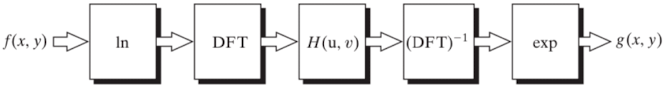
\includegraphics[width=\columnwidth]{homomorphic-filtering.png}
\end{figure}

위와 같은 일련의 과정을 homorphic filtering이라고 하며, 이미지의 조명과 반사광을 구분함으로써 조명을 조절하거나 반사를 조절할 수 있게 해준다.

Illumination-Reflectance Model: 조명(illumination)은 천천히, 반사(reflectance)는 빠르게 변한다. 즉, 전반적으로 밝기가 서서히 바뀌는 것은 illumination(저주파), 자주 바뀌는 것을 reflectance(고주파)로 생각할 수 있음. 그래서 아래와 같은 필터를 만들 수 있다.
$$H(u, v) = (\gamma_H - \gamma_L)^{[1 - e^{-c [{D^2(u, v) \over D_0^2}]}]} + \gamma_L$$
가우시안을 뒤집고, 범위를 조정한 다음 아래로 평행이동한 것. $D_0$는 폭을 조정. 조명이 빨리 변화하게 하려면 크게, 천천히 변화하게 하려면 작게. 샤프닝 효과가 있다.

\subsubsection{Selective Filtering}

특정 직사강형 영역의 중심부에 미리 정의된 범위의 주파수를 차단하거나 통과시켜 선택된 부분만 필터링할 수 있음.
